\documentclass{llncs}
\usepackage{etex}

\usepackage{xcolor}
\usepackage{enumitem,amsmath,amssymb}
%\usepackage{breakurl}    % used for \url and \burl
\usepackage{url}
\usepackage[linesnumbered,boxed,noline,noend]{algorithm2e}
\def\defaultHypSeparation{\hskip.1in}

\usepackage{tikz}
\usepackage{subfig}
\usepackage{array,booktabs,multirow}
\usepackage{placeins}

\usepackage{logictools}
\usepackage{prooftheory}
\usepackage{comment}
\usepackage{mathenvironments}
\usepackage{drawproof}
\usepackage{bussproofs}
\usepackage{tensor}
\usepackage{mathtools}
\usepackage{amsmath}

\usepackage{graphicx}
%\usepackage{caption}
%\usepackage{subcaption}

\renewcommand{\topfraction}{0.85}
\renewcommand{\textfraction}{0.1}
\renewcommand{\floatpagefraction}{0.75}


\newcommand{\freevar}[1]{\mathrm{FV}(#1)}

\newcommand{\Vertices}[1]{V_{#1}}
\newcommand{\Edges}[1]{E_{#1}}
\newcommand{\Conclusion}[1]{\clause_{#1}}

\newcommand{\axiom}[1]{\widehat{#1}}
\newcommand{\n}{v}
\newcommand{\raiz}[1]{\rho(#1)}

\newcommand{\pedge}[3]{\ensuremath{\raiz{#1} \xrightarrow{#2} \raiz{#3}}}


\newcommand\inlineeqno{\stepcounter{equation}\ (\theequation)}


% Contraction
\newcommand{\con}[3]{\lfloor #1 \rfloor_{#2}^{#3}}

% Resolution
%\newcommand{\res}[6]{#1 \tensor[^{#2}_{#3}]{\odot}{^{#4}_{#5}} #6}
%\newcommand{\res}[6]{#1 \prescript{#2}{#3}{\odot^{#4}_{#5}} #6}

\newcommand{\res}[4]{\mathrel{\operatorname*{\odot}_{#1 #3}^{#2 #4}}}

\title{Partial Regularization of\\ First-Order Resolution Proofs\\
(Experimental/Tool Paper)}

\author{
  Jan Gorzny\inst{1}
  \thanks{Supported by the Google Summer of Code 2014 program.}
  \and 
  Bruno Woltzenlogel Paleo\inst{2,3}
  %\thanks{Supported by the Austrian Science Fund, project P24300.}
}

\authorrunning{J.\~Gorzny \and B.\~Woltzenlogel Paleo}

\institute{
  \email{jgorzny@uvic.ca}, University of Victoria, Canada
  \and 
  \email{bruno@logic.at}, Vienna University of Technology, Austria
  \and 
  Australian National University
}




\begin{document}

\maketitle


\begin{abstract}
This paper describes the generalization of the 
proof compression algorithm
\RecyclePivotsIntersection 
%\texttt{RecyclePivots\-WithIntersection}
from propositional to first-order logic. The generalized algorithm performs partial regularization of resolution proofs containing resolution and factoring inferences with \emph{unification}, as generated by many automated theorem provers. An empirical evaluation of the generalized algorithm and its combinations with \SFOLowerUnits is also presented.
\end{abstract}


\setcounter{footnote}{0}

\section{Introduction} 

First-order automated theorem provers, commonly based on resolution and superposition calculi, have recently achieved a high degree of maturity. Proof production is a key feature that has been gaining importance, since proofs are crucial for applications that require certification of a prover's answers or information extractable from proofs (e.g. unsat cores, interpolants, instances of quantified variables). Nevertheless, proof production is non-trivial \cite{SchulzAPPA}, and the best, most efficient provers do not necessarily generate the best, least redundant proofs.

For proofs using propositional resolution generated by SAT- and SMT-solvers, there is a wide variety of proof compression techniques. Algebraic properties of the resolution operation that might be useful for compression were investigated in \cite{bwp10}.
Compression algorithms based on rearranging and sharing chains of resolution inferences have been
developed in \cite{Amjad07} and \cite{Sinz}.  Cotton \cite{CottonSplit} proposed an algorithm that
compresses a refutation by repeatedly splitting it into a proof of a heuristically chosen literal $\ell$
and a proof of $\dual{\ell}$, and then resolving them to form a new refutation.  The {\ReduceReconstruct} algorithm \cite{RedRec} searches for locally redundant
subproofs that can be rewritten into subproofs of stronger clauses and with fewer resolution steps.
A linear time proof compression algorithm based on partial
regularization was proposed in \cite{RP08} and improved in \cite{LURPI}.

In contrast, there has been much less work on simplifying first-order proofs. For tree-like sequent calculus proofs, algorithms based on cut-introduction \cite{BrunoLPAR,Hetzl} have been proposed. However, converting a DAG-like resolution or superposition proof, as usually generated by current provers, into a tree-like sequent calculus proof may increase the size of the proof. For arbitrary proofs in the TPTP \cite{TPTP} format (including DAG-like first-order resolution proofs), there is a simple algorithm \cite{LPARCzech} that looks for terms that occur often in any TSTP \cite{TPTP} proof and introduces abbreviations for these terms. 


The work reported in this paper is part of a new trend that aims at lifting successful propositional proof compression algorithms to first-order logic. Our first target was the propositional {\LowerUnits} algorithm, which delays resolution steps with unit clauses, resulting in the
{\SFOLowerUnits} 
({\GFOLU}) algorithm \cite{GFOLU}. Here we continue this line of research by lifting the 
%\RecyclePivotsIntersection 
\texttt{Recycle\-PivotsWithIntersection}
({\RPI}) algorithm \cite{LURPI}, which is an improvement of the \texttt{RecyclePivots} ({\RP}) algorithm \cite{RP08}, providing better compression on proofs where nodes have several children. 

%TODO: edit this again
Section \ref{sec:res} introduces the first-order resolution calculus and the notations used in this paper. Section \ref{sec:Challenges} discusses the challenges that arise in the first-order case (mainly due to unification), which are not present the propositional case. Section \ref{sec:FORPI} describes an algorithm that overcomes these challenges. Section \ref{sec:exp} presents experimental results obtained by applying this algorithm, and its combinations with {\GFOLU}, on hundreds of proofs generated with the {\SPASS} theorem prover. Section \ref{sec:conclusion} concludes the paper.



\section{The Resolution Calculus}

We assume that there are infinitely many variable symbols (e.g. $X$, $Y$, $Z$, $X_1$, $X_2$, \ldots), constant symbols (e.g. $a$, $b$, $c$, $a_1$, $a_2$, \ldots), function symbols of every arity (e.g $f$, $g$, $f_1$, $f_2$, \ldots) and predicate symbols of every arity (e.g. $p$, $q$, $p_1$, $p_2$,\ldots). A \emph{term} is any variable, constant or the application of an $n$-ary function symbol to $n$ terms.
An \emph{atomic formula} (\emph{atom}) is the application of an $n$-ary predicate symbol to $n$ terms. A \emph{literal} is an atom or the negation of an atom. The
\emph{complement} of a literal $\ell$ is denoted $\dual{\ell}$ (i.e. for any atom $p$,
$\dual{p} = \neg p$ and $\dual{\neg p} = p$). The set of all literals is denoted $\mathcal{L}$. A
\emph{clause} is a multiset of literals. $\bot$ denotes the \emph{empty clause}. A \emph{unit clause} is clause with a single literal. Sequent notation is used for clauses (i.e. $p_1,\ldots,p_n \seq q_1,\ldots, q_m$ denotes the clause $\{ \neg p_1,\ldots, \neg p_n, q_1, \ldots, q_m \}$).
$\freevar{t}$ (resp. $\freevar{\ell}$, $\freevar{\clause}$) denotes the set of variables in the term $t$ (resp. in the literal $\ell$ and in the clause $\clause$).
A \emph{substitution} $\{ X_1\backslash t_1, X_2 \backslash t_2, \ldots \}$ is a mapping from variables $\{ X_1, X_2, \ldots \}$ to, respectively, terms $\{t_1, t_2, \ldots \}$. The application of a substitution $\sigma$ to a term $t$, a literal $\ell$ or a clause $\clause$ results in, respectively, the term $t \sigma$, the literal $\ell \sigma$ or the clause $\clause \sigma$, obtained from $t$, $\ell$ and $\clause$ by replacing all occurrences of the variables in $\sigma$ by the corresponding terms in $\sigma$. The set of all substitutions is denoted $\mathcal{S}$. A \emph{unifier} of a set of literals is a substitution that makes all literals in the set equal.
A \emph{resolution proof} is a directed acyclic graph of clauses where the edges correspond to the inference rules of resolution and contraction (as explained in detail in Definition \ref{def:proof}). A \emph{resolution refutation} is a resolution proof with root $\bot$.


\begin{definition}[First-Order Resolution Proof] 
\label{def:proof} \hfill \\
A directed acyclic graph $\langle V, E, \clause \rangle$, where $V$ is a set of nodes and $E$ is a
set of edges labeled by literals and substitutions (i.e. $E \subset V \times \mathcal{L} \times \mathcal{S} \times V$ and $\n_1
\xrightarrow[\sigma]{\ell} \n_2$ denotes an edge from node $\n_1$ to node $\n_2$ labeled by the literal $\ell$ and the substitution $\sigma$), is a
proof of a clause $\clause$ iff it is inductively constructible according to the following cases:
%
\begin{itemize}
  \item \textbf{Axiom:} If $\Gamma$ is a clause, $\axiom{\Gamma}$ denotes some proof $\langle \{ \n \}, \varnothing,
    \Gamma \rangle$, where $\n$ is a new (axiom) node.
  \item \textbf{Resolution:} If $\psi_L$ is a proof $\langle V_L, E_L, \clause_L \rangle$ with $\ell_L \in \clause_L$ and
    $\psi_R$ is a proof $\langle V_R, E_R, \clause_R \rangle$ with $\ell_R \in \clause_R$, and 
    $\sigma_L$ and $\sigma_R$ are substitutions such that
    $\ell_L \sigma_L = \dual{\ell_R} \sigma_R$ and
    $\freevar{\left( \clause_L \setminus \left\{ \ell_L \right\} \right) \sigma_L} \cap 
     \freevar{\left( \clause_R
                    \setminus \left\{ \ell_R \right\} \right) \sigma_R} = \emptyset$, 
    then
    $\psi_L \res{\ell_L}{\sigma_L}{\ell_R}{\sigma_R} \psi_R$ denotes a proof $\langle V, E, \Gamma \rangle$ s.t.
    \begin{align*}
      V &= V_L \cup V_R \cup \{\n \} \\
      E &= E_L \cup E_R \cup
                    \left\{ \raiz{\psi_L} \xrightarrow[\sigma_L]{\ell_L} \n, 
                            \raiz{\psi_R} \xrightarrow[\sigma_R]{\ell_R} \n \right\} \\
     \Gamma &= \left( \clause_L \setminus \left\{ \ell_L \right\} \right) \sigma_L \cup \left( \clause_R
                    \setminus \left\{ \ell_R \right\} \right) \sigma_R 
    \end{align*}
    where $\n$ is a new (resolution) node and $\raiz{\varphi}$ denotes the root node of $\varphi$.
  \item \textbf{Contraction:} If $\psi'$ is a proof $\langle V', E', \clause' \rangle$ and $\sigma$ is a unifier of $\{\ell_1, \ldots \ell_n\}$ with $\{\ell_1, \ldots \ell_n\} \subseteq \clause'$, then, letting $\ell = \ell_k \sigma$ (for any $k \in \{1,\ldots, n\}$), $\con{\psi}{\sigma}{\ell}$ denotes a proof $\langle V, E, \Gamma \rangle$ s.t.
    \begin{align*}
      V &= V' \cup \{\n \} \\
      E &= E' \cup \{ \raiz{\psi'} \xrightarrow[\sigma]{\ell} \n \} \\
     \Gamma &= (\clause' \setminus \{ \ell_1, \ldots \ell_n \} ) \sigma \cup \{ \ell \}
    \end{align*}
    where $\n$ is a new (contraction) node and $\raiz{\varphi}$ denotes the root node of $\varphi$.
  \qed
\end{itemize}
\end{definition}




\noindent
If $\psi = \varphi_L \odot_{\ell} \varphi_R$, then $\varphi_L$ and $\varphi_R$ are \emph{direct
subproofs} of $\psi$ and $\psi$ is a \emph{child} of both $\varphi_L$ and $\varphi_R$. The
transitive closure of the direct subproof relation is the \emph{subproof} relation. A subproof which
has no direct subproof is an \emph{axiom} of the proof.
%
$\Vertices{\psi}$, $\Edges{\psi}$ and $\Conclusion{\psi}$
denote, respectively, the nodes, edges and proved clause (conclusion) of $\psi$.


\section{The Propositional Algorithm}

{\RPI} (formally defined in Appendix \ref{Section:RPI}) removes \emph{irregularities}, which are resolution inferences with a node $\eta$ when the resolved literal (a.k.a. \emph{pivot}) occurs as the pivot of another inference located below in the path from $\eta$ to the root of the proof. In the worst case, regular resolution proofs can be exponentially bigger than irregular ones, but {\RPI} takes care of regularizing the proof only partially, removing inferences only when this does not enlarge the proof.

%ToDo: Informal textual description of the propositional algorithm, explaining what safe literals are. 
{\RPI} traverses the proof twice. On the first traversal (bottom-up), it stores for each node a set of \emph{safe literals} that are resolved in all paths below it in the proof or that occur in the root clause of the proof. If one of the node's resolved literals belongs to the set of safe literals, then it is possible to \emph{regularize} the node by replacing it by the parent containing the safe literal. To do this replacement efficiently, the replacement is postponed by marking the other parent as a \texttt{deletedNode}. Then, on a single second traversal (top-down), regularization is performed: any node that has a parent node marked as a \texttt{deletedNode} is replaced by its other parent.
%Refer reader to the CADE 2011 paper (where RPI is described) for a formal description of the propositional algorithm. 
% contains a formal description of {\RPI} (taken from \cite{LURPI}).
%Consider adding the formal description to an appendix in this paper, for the convenience of the reviewer.

The {\RPI} and the {\RP} algorithms differ from each other mainly in the
computation of the safe literals of a node that has many children. While the former 
returns the intersection as shown in Algorithm~\ref{algo:SetSafeLiterals}, the latter
returns the empty set. 
Moreover, while in {\RPI} the safe literals of the root node contain all the literals of the root clause, in {\RP} the root node is always assigned an empty set of literals. 


\section{First-Order Challenges}\label{sec:Challenges}


In this section, we describe challenges that have to be overcome in order to successfully adapt {\RPI} to the first-order case. The first example illustrates the need to take unification into account. The other two examples discuss complex issues that can arise when unification is take into account in a naive way.

%straightforward example
\begin{example}\label{ex:unif} 
Consider the following irregular proof $\psi$. Naively computed, the safe literals for $\eta_3$ are $\{ \vdash q(c), ~ p(a,X)\}$. $\eta_1$ and $\eta_5$ and these two literals are unifiable. Further, the safe literals for $\eta_1$ includes $\eta_5$. Thus the proof can be regularized by recycling $\eta_1$.

\begin{footnotesize}
\begin{prooftree}
\def\e{\mbox{\ $\vdash$\ }}
\AxiomC{$\eta_1$: \e $p(W,X)$}
\AxiomC{$\eta_2$: $p(W,X)$ \e $q(c)$}
\BinaryInfC{$\eta_3$: \e $q(c)$}
\AxiomC{$\eta_4$: $q(c)$ \e $p(a,X)$}
\BinaryInfC{$\eta_5$: \e $p(a,X)$}
\AxiomC{$\eta_6$: $p(Y,b)$ \e }
\BinaryInfC{$\psi$: $\bot$}
\end{prooftree}
\end{footnotesize}

\noindent
Regularization of the proof by recycling $\eta_1$ results in deleting the edge between $\eta_2$ and $\eta_3$, which in turn replaces $\eta_3$ by $\eta_1$. Since $\eta_1$ cannot be resolved against $\eta_4$, and $\eta_1$ contained safe literals, $\eta_5$ is replaced by $\eta_1$. The result is the much shorter proof below.

\begin{footnotesize}
\begin{prooftree}
\def\e{\mbox{\ $\vdash$\ }}
\AxiomC{$\eta_1$: \e$p(W,X)$}
\AxiomC{$\eta_6$: $p(Y,b)$\e}
\BinaryInfC{$\psi'$: $\bot$}
\end{prooftree}
\end{footnotesize}

\noindent
Unlike in the propositional case, where the pivots and their corresponding safe literal list are all syntactically equal, in the first-order case, this is not necessarily the case. As illustrated above, $p(W,X)$ and $p(a,X)$ are not syntactically equal. Nevertheless, they are unifiable, and the proof can be regularized.
\end{example}

%unification necessary example
\begin{example}\label{ex:pairwise}

There are cases, as shown below, that require more careful care when attempting to regularize. Again, naively computed the safe literals for $\eta_3$ are $\{ \vdash q(c), ~ p(a,X)\}$, and so $\eta_1$ and $\eta_2$ appear to be candidates for regularization. 

\begin{footnotesize}
\begin{prooftree}
\def\e{\mbox{\ $\vdash$\ }}
\AxiomC{$\eta_1$: \e $p(a,c)$}
\AxiomC{$\eta_2$: $p(a,c)$ \e $q(c)$}
\BinaryInfC{$\eta_3$: \e $q(c)$}
\AxiomC{$\eta_4$: $q(c)$ \e $p(a,X)$}
\BinaryInfC{$\eta_5$: \e $p(a,X)$}
\AxiomC{$\eta_6$: $p(Y,b)$ \e }
\BinaryInfC{$\psi$: $\bot$}
\end{prooftree}
\end{footnotesize}


\noindent
However, if we attempt to regularize the proof, the same series of actions as in Example \ref{ex:unif} would result in the following resolution, which cannot be completed.

\begin{footnotesize}
\begin{prooftree}
\def\e{\mbox{\ $\vdash$\ }}
\AxiomC{$\eta_1$: \e$p(a,c)$}
\AxiomC{$\eta_6$: $p(Y,b)$\e}
\BinaryInfC{$\psi'$: ??}
\end{prooftree}
\end{footnotesize}

\end{example}

\noindent
The observations above lead to the idea of requiring pivots to satisfy the following property before collecting them to be reused.

\begin{definition}
\label{prop:pair}
Let $\eta$ be a clause with literal $\ell'$ with corresponding safe literal $\ell$ which is resolved against literals $\ell_1$, \ldots, $\ell_n$ in a proof $\psi$. $\eta$ is said to satisfy the \emph{pre-regularization unifiability property} in $\psi$ if $\ell_1$,\ldots,$\ell_n$, and $\dual{\ell'}$ are unifiable.
\end{definition}

\noindent
One technique to ensure this property is met is to apply the unifier of a resolution to each resolvent before computing the safe literals. In the case of Example \ref{ex:pairwise}, this would result in $\eta_1$ having the safe literals $\{ \vdash q(c),~p(a,b)\}$, and now it is clear that the literal in $\eta_1$ is not safe.

%TODO: continue from here
%extra check example
\begin{example}\label{ex:unifcheck}
Due to complications with unification, there are also cases where satisfying the pre-regularization unifiability property is not sufficient to attempt regularization. Consider the proof of $\psi$ below. After collecting the safe literals, $\eta_3$'s safe literals are $\{q(T,V),p(c,d)\vdash q(f(a,e),c)\}$.

\begin{footnotesize}
\begin{prooftree}
\def\e{\mbox{\ $\vdash$\ }}
\AxiomC{$\eta_8$: $q(f(a,e),c)\e$\hspace{-1cm}}
\AxiomC{$\eta_6$: $\e p(c,d)$\hspace{-4.5cm}}
\AxiomC{$\eta_1$: $p(U,V)\e q(f(a,V),U)$}
\AxiomC{$\eta_2$: $q(f(a,X),Y),q(T,X)\e q(f(a,Z),Y)$}
\BinaryInfC{$\eta_3$: $p(U,V),Q(T,V)\e q(f(a,Z),U)$\hspace{-3.5cm}}
\AxiomC{\hspace{-1.5cm} $\eta_4$: $\e q(R,S)$}
\BinaryInfC{$\eta_5$: $p(U,V)\e q(f(a,Z),U)$}
\BinaryInfC{$\eta_7$: $\e q(f(a,Z),c)$}
\BinaryInfC{$\psi$: $\bot$}
\end{prooftree}
\end{footnotesize}

\noindent
Since $q(f(a,X),Y) \in \eta_2$ and $q(T,V)$ (in $\eta_3$'s safe literals) are unifiable, regularization would be attempted. However, in this case, we would mark the edge between $\eta_2$ and $\eta_3$ for deletion, and as a result, $\eta_3$ will be replaced with $\eta_1$. $\eta_1$ does not contain the required pivot for $\eta_5$, and so $\eta_5$ is also replaced with $\eta_1$, and resolution is attempted before $\eta_1$ and $\eta_6$, which results in $\eta_7'$, and an inability to complete the proof, as shown below.

\begin{footnotesize}
\begin{prooftree}
\def\e{\mbox{\ $\vdash$\ }}
\AxiomC{$\eta_8$: $Q(f(ae)c)\e$}
\AxiomC{$\eta_6$: $\e P(cd)$}
\AxiomC{$\eta_1$: $P(UV)\e Q(f(aV)U)$}
\BinaryInfC{$\eta_7'$: $\e Q(f(ad)c)$}
\BinaryInfC{$\psi'$: ??}
\end{prooftree}
\end{footnotesize}

In order to avoid these scenarios, we perform an additional check during edge deletion. The node $\eta*$ which will replace a resolution $\eta$ (because $\eta$ would have a deleted parent), must be entirely contained, via unification which modifies only $\eta^*$'s variables, in the safe literals of $\eta$. In the case of this example, $\eta_1$ would not satisfy this property: in order to unify with $\eta_3$'s safe literals, it would be necessary to send $V\rightarrow Z$ due to $\eta_1$'s second literal, but leave $V$ unchanged due $\eta_1$'s first literal, which is not possible. Note that this check is not necessary in the propositional case, as the replacement node would be contained exactly in the set of safe literals.

\end{example}


%intersection example?
\section{First-Order RecyclePivotsWithIntersection}
\label{sec:FORPI}
%TODO: this section
This section presents {\FirstOrderRPI} ({\FORPI}), Algorithm \ref{algo:FORPI}, a first order generalization of {\RPI}. 
%which aims to compress irregular proofs. 
%Recall that \RecyclePivotsIntersection is a modification of the \texttt{RecyclePivots} algorithm, %described in  \cite{Bar-IlanFuhrmannHooryShachamStrichman2009Linear-time-reductions-of-resolution-proofs}, from which it derives its name. 
%and \RecyclePivotsIntersection provides better compression on proofs where nodes have several children, when compared to \texttt{RecyclePivots}. Through a small modification to our algorithm (described later), a first order generalization of \texttt{RecyclePivots} is also possible.
%Our generalization, Algorithm~\ref{algo:FORPI}. 
It follows the propositional idea of traversing the proof in a bottom-up manner, storing for every node a set of \emph{safe literals} that get resolved in all paths below it in the proof (or that already occurred in the root clause of the original proof). If one of the node's resolved literals can be unified to a literal in the set of safe literals, then it may be possible to regularize the node by replacing it by one of its parents. 

%TODO: move to intro?
%Although in the worst case full regularization can increase the proof length exponentially \cite{Tseitin1983On-The-Complexity-of-Proofs-in-Propositional-Logics}, these algorithms show that many irregular proofs can have their length decreased if a careful partial regularization is performed. 

\newcommand{\la}{\leftarrow}


\begin{algorithm}[bt]
\begin{footnotesize}
\SetKwInOut{Input}{input}\SetKwInOut{Output}{output}
\SetKwData{units}{unitsQueue}
\SetKwData{fixedUnits}{fixedUnitsQueue}

\Input{A first-order proof $\psi$}
\Output{A possibly less-irregular first-order proof $\psi'$}

\BlankLine

$\psi'$ $\la$ $\psi$\;
traverse $\psi'$ bottom-up and \ForEach{node $\eta$ in $\psi'$}{
   \If{$\eta$ is a resolvent node}{
     setSafeLiterals($\eta$) \;
     regularizeIfPossible($\eta$)
   }
  }
$\psi'$ $\la$ fix($\psi'$) \;
\Return {$\psi'$}\;
\caption{\label{algo:FORPI} \texttt{\FORPI}}
\end{footnotesize}
\end{algorithm}





%TODO: re-write -- taken from FORPI paper
In the propositional case, regularization of a node replaces it by the parent whose clause contains the resolved literal that is safe. In the first order case, because unification introduces complications like those seen in Example \ref{ex:unifcheck}, we ensure that the replacement parent is (possibly after unification) contained entirely in the safe literals. This ensures that the remainder of the proof does not expect a variable to be unified to different values simultaneously. After regularization, all nodes below the regularized node may have to be fixed. 
Similar to {\RPI}, instead of replacing the irregular node by one of its parents immediately, 
its other parent is replaced by \texttt{deletedNodeMarker}, as shown in Algorithm~\ref{algo:Regularize}.
As in the propositional case, fixing of the proof is postponed to another (single) traversal, as regularization proceeds bottom up and only nodes below a regularized node may require fixing.
During fixing, the irregular node is actually replaced by the parent that is not \texttt{deletedNodeMarker}.


%Unchanged from propositional case? %TODO: or should the $\in$ relation be unification?
\begin{algorithm}[bt]
\begin{footnotesize}

\SetKwInOut{Input}{input}\SetKwInOut{Output}{output}
\SetKwData{units}{unitsQueue}
\SetKwData{fixedUnits}{fixedUnitsQueue}

\Input{A node $\psi=\psi_L  \res{\ell_L}{\sigma_L}{\ell_R}{\sigma_R} \psi_R$}
\Output{nothing (but the proof containing $\psi$ may be changed)}

\BlankLine
    \uIf{$\exists \sigma$  and $l \in \psi${\upshape.safeLiterals} such that $\sigma l = l_R$ or $l=\sigma l_R$}{
     \uIf{$\exists \sigma$ such that $\sigma\psi_R\subseteq\psi${\upshape.safeLiterals}} {
      replace $\psi_L$ of $\eta$ by \texttt{deletedNodeMarker} \;
      mark $\psi$ as regularized
}
    }
    \ElseIf{$\exists \sigma$  and $l \in \psi${\upshape.safeLiterals} such that $\sigma l = l_L$ or $l=\sigma l_L$}{
     \uIf{$\exists \sigma$ such that $\sigma\psi_L\subseteq\psi${\upshape.safeLiterals}} {
      replace $\psi_R$ by \texttt{deletedNodeMarker} \;
      mark $\psi$ as regularized
}
    }
\caption{\label{algo:Regularize} \texttt{regularizeIfPossible}}
\end{footnotesize}
\end{algorithm}


\begin{algorithm}[bt]
\begin{footnotesize}

\SetKwInOut{Input}{input}\SetKwInOut{Output}{output}
\SetKwData{units}{unitsQueue}
\SetKwData{fixedUnits}{fixedUnitsQueue}

\Input{A first order resolution node $\psi$}
\Output{nothing (but the node $\psi$ gets a set of safe literals)}

\BlankLine

    \uIf{$\psi$ is a root node with no children}{
      $\psi$.safeLiterals $\la$ $\psi$.clause  
    }
    \Else{
      \ForEach{$\psi'$ $\in$ $\psi${\upshape.children}}{
        \uIf{$\psi'$ is marked as regularized}{ 
          safeLiteralsFrom($\psi'$) $\la$ $\psi'$.safeLiterals \;}
%        \uElseIf{$\eta$ is left parent of $\eta'$}{ 
          \uElseIf{$\psi' = \psi  \res{\ell_L}{\sigma_L}{\ell_R}{\sigma_R} \psi_R$ for some $\psi_R$}{ 
        	safeLiteralsFrom($\psi'$) $\la$ $\psi'$.safeLiterals $\cup$ \{ $\sigma_R l_R \}$ %\;
        }
        \ElseIf{$\psi' = \psi_L  \res{\ell_L}{\sigma_L}{\ell_R}{\sigma_R} \psi$ for some $\psi_L$}{ 
	safeLiteralsFrom($\psi'$) $\la$ $\psi'$.safeLiterals $\cup$ \{ $\sigma_L l_L \}$%\;
        }
      }
      $\psi$.safeLiterals $\la$ $\bigcap_{\psi' \in \psi\textrm{.children}}$ safeLiteralsFrom($\psi'$)
    }
\caption{\label{algo:SetSafeLiterals} \texttt{setSafeLiterals}}
\end{footnotesize}
\end{algorithm}


%original
%\begin{algorithm}[bt]
%\begin{footnotesize}
%\SetKwInOut{Input}{input}\SetKwInOut{Output}{output}
%\SetKwData{units}{unitsQueue}
%\SetKwData{fixedUnits}{fixedUnitsQueue}
%\Input{A node $\eta$}
%\Output{nothing (but the node $\eta$ gets a set of safe literals)}
%\BlankLine
%    \uIf{$\eta$ is a root node with no children}{
%      $\eta$.safeLiterals $\la$ $\eta$.clause  
%    }
%    \Else{
%      \ForEach{$\eta'$ $\in$ $\eta${\upshape.children}}{
%        \uIf{$\eta'$ is marked as regularized}{ 
%          safeLiteralsFrom($\eta'$) $\la$ $\eta'$.safeLiterals \;}
%        \uElseIf{$\eta$ is left parent of $\eta'$}{ 
%        	safeLiteralsFrom($\eta'$) $\la$ $\eta'$.safeLiterals $\cup$ \{ $\eta'$.rightResolvedLiteral \} \;
%        }
%        \ElseIf{$\eta$ is right parent of $\eta'$}{ 
%			safeLiteralsFrom($\eta'$) $\la$ $\eta'$.safeLiterals $\cup$ \{ $\eta'$.leftResolvedLiteral \} \;
%        }
%      }
%      $\eta$.safeLiterals $\la$ $\bigcap_{\eta' \in \eta\textrm{.children}}$ safeLiteralsFrom($\eta'$)
%    }
%\caption{\label{algo:SetSafeLiterals} \texttt{setSafeLiterals}}
%\end{footnotesize}
%\end{algorithm}

%The set of safe literals of a node $\eta$ can be computed from the set of safe literals of its children (cf.\ Algorithm~\ref{algo:SetSafeLiterals}). In the case when $\eta$ has a single child $\varsigma$, the safe literals of $\eta$ are simply the safe literals of $\varsigma$ together with the resolved literal $p$ of $\varsigma$ belonging to $\eta$ ($p$ is safe for $\eta$, because whenever $p$ is propagated down the proof through $\eta$, $p$ gets resolved in $\varsigma$). It is important to note, however, that if $\varsigma$ has been marked as regularized, it will eventually be replaced by $\eta$, and hence $p$ should not be added to the safe literals of $\eta$. In this case, the safe literals of $\eta$ should be exactly the same as the safe literals of $\varsigma$. When $\eta$ has several children, the safe literals of $\eta$ w.r.t. a child $\varsigma_i$ contain literals that are safe on all paths that go from $\eta$ through $\varsigma_i$ to the root. For a literal to be safe for all paths from $\eta$ to the root, it should therefore be in the intersection of the sets of safe literals w.r.t. each child.

The {\RPI} and the {\RP} algorithms differ from each other mainly in the
computation of the safe literals of a node that has many children. While the former 
returns the intersection as shown in Algorithm~\ref{algo:SetSafeLiterals}, the latter
returns the empty set. 
Further, while in {\RPI} the safe literals of the root node contain all the literals of the root clause, in {\RP} the root node is always assigned an empty set of literals. 
This is easy accomplished in the first order case by changing lines 11 and 2, respectively, of Algorithm~\ref{algo:SetSafeLiterals}.
This makes a difference only when the proof is not a refutation.

The set of safe literals for a node $\psi$ is computed from the set of safe literals of its children (cf.\ Algorithm~\ref{algo:SetSafeLiterals}), similar to the propositional case, but additionally applies unifiers to the resolved pivots (cf. Example \ref{ex:pairwise}).


%Note that during a traversal of the proof,  the lines from 5 to 10 in Algorithm~\ref{algo:SetSafeLiterals} are executed as many times as the number of edges in the proof.  Since every node has at most two parents, the number of edges is at most twice the number of nodes.  Therefore, during a traversal of a proof with $n$ nodes, lines from 5 to 10 are executed at most $2n$ times, and the algorithm remains linear. In our prototype implementation, the sets of safe literals are instances of Scala's  \texttt{mutable.HashSet} class. Being mutable, new elements can be added efficiently. And being HashSets, membership checking is done in constant time in the average case, and set intersection (line 12) can be done in $O(k.s)$, where $k$ is the number of sets and $s$ is the size of the smallest set.





\section{Experiments} \label{sec:exp}
A prototype\footnote{Source code available at \url{https://github.com/jgorzny/Skeptik}} version of {\FORPI} has been implemented in the functional programming language Scala as part of the \skeptik
 library. %\footnote{\url{https://github.com/Paradoxika/Skeptik}}. 
%{\SFOLowerUnits} prototype was developed earlier for the same system \cite{}.
Evaluation of this algorithm was performed on the same 308 real first-order proofs generated to evaluate {\GFOLU}, and for consistency, the same system and metrics were used (see \cite{GFOLU}).

Figure \ref{fig:ex} (a) shows the compression results of applying {\FORPI} and {\GFOLU} to the same proof (in both application orders), as well as each of these algorithms individually. 
%Unsurprisingly, applying both algorithms generally does better than either algorithm alone. 
With this data, {\FORPI} compresses provides some compression to the original proofs, although {\GFOLU} is responsible for most of the compression. {\FORPI} compresses only three proofs already compressed by {\GFOLU}.
{\RPI} performs best when the proofs are tall; {\FORPI} will likely perform similarly. However, the proofs in this data set are relatively short, and those compressed by {\GFOLU} first are even shorter. Thus, the performance of {\FORPI} is not surprising.

Figure \ref{fig:ex} (b) shows that the order of compression may matter less than in than in the propositional case, although more data is needed for confirmation. The number of points above and below the main diagonal are the same; however, the points below may simply be the result of {\GFOLU} being more likely to compress such short proofs. If so, that would imply that running {\FORPI} after {\GFOLU} is more successful, which would be consistent with propositional results for these algorithms.
%Running {\FORPI} after {\GFOLU} shows some compression that...
%This is consistent with propositional results for these algorithms.

%Before evaluating this algorithm, we first generated several benchmark proofs. This was done by executing the {\SPASS}\footnote{\url{http://www.spass-prover.org/}} theorem prover on 2280 real first-order problems without equality of the TPTP Problem Library \footnote{\url{http://www.cs.miami.edu/{\textasciitilde}tptp/}} (among them, 1032 problems are known to be unsatisfiable). In order to generate pure resolution proofs, most advanced inference rules used by {\SPASS}  were disabled. The Euler Cluster at the University of Victoria\footnote{\url{https://rcf.uvic.ca/euler.php}} was used and the time limit was 300 seconds per problem. Under these conditions, {\SPASS} was able to generate 308 proofs. 


%The proofs generated by {\SPASS} were small (with lengths from 3 to 49). These proofs are specially small in comparison with the typical proofs generated by SAT- and SMT-solvers, which usually have from a few hundred to a few million nodes. The number of proofs (compressed and uncompressed) per length is shown in Figure \ref{fig:ex} (b). Uncompressed proofs are those which had either no lowerable units to lower or for which \SFOLowerUnits failed and returned the original proof. Such failures occurred on only 14 benchmark proofs. Among the smallest of the 308 proofs, very few proofs were compressed. This is to be expected, since the likelihood that a very short proof contain a lowerable unit (or even merely a unit with more than one child) is low. The proportion of compressed proofs among longer proofs is, as expected, larger, since they have more nodes and it is more likely that some of these nodes are lowerable units. 13 out of 18 proofs with length greater than or equal to 30 were compressed. 

%Figure \ref{fig:ex} (a) shows a box-whisker plot of compression ratio with proofs grouped by length and whiskers indicating minimum and maximum compression ratio achieved within the group. Besides the median compression ratio (the horizontal thick black line), the chart also shows the mean compression ratios for all proofs of that length and for all compressed proofs (the red cross and the blue circle). In the longer proofs (length greater than 34), the median and the means are in the range from 5\% to 15\%, which is satisfactory in comparison with the total compression ratio of 7.5\% that has been measured for the propositional {\LowerUnits} algorithm on much longer propositional proofs \cite{Boudou}.

%Figure \ref{fig:ex} (c) shows a scatter plot comparing the length of the input proof against the length of the compressed proof. For the longer proofs (circles in the right half of the plot), it is often the case that the length of the compressed proof is significantly lesser than the length of the input proof.

%Figure \ref{fig:ex} (d) plots the cumulative original and compressed lengths of all benchmark proofs (for an x-axis value of $k$, the cumulative curves show the sum of the lengths of the shortest $k$ input proofs). The total cumulative length of all original proofs is 4429 while the cumulative length of all proofs after compression is 3929. This results in a total compression ratio of 11.3\%, which is impressive, considering that the inclusion of all the short proofs (in which the presence of lowerable units is a priori unlikely) tends to decrease the total compression ratio. For comparison, the total compression ratio considering only the 100 longest input proofs is 18.4\%.

%Figure \ref{fig:ex} also indicates an interesting potential trend. The gap between the two cumulative curves seems to grow superlinearly. If this trend is extrapolated, progressively larger compression ratios can be expected for longer proofs. This is compatible with Theorem 10 in \cite{LURPI}, which shows that, for proofs generated by eagerly resolving units against all clauses, the propositional {\LowerUnits} algorithm can achieve quadratic assymptotic compression. SAT- and SMT-solvers based on CDCL (Conflict-Driven Clause Learning) avoid eagerly resolving unit clauses by dealing with unit clauses via boolean propagation on a conflict graph and extracting subproofs from the conflict graph with every unit being used at most once per subproof (even when it was used multiple times in the conflict graph). Saturation-based automated theorem provers, on the other hand, might be susceptible to the eager unit resolution redundancy described in Theorem 10 \cite{LURPI}. This potential trend would need to be confirmed by further experiments with more data (more proofs and longer proofs).


%TODO: change time
%{\SPASS} required approximately 40 minutes (running on a cluster and proof generation time for each problem) to solve the generated proofs. The total time for {\GFOLU} and {\FORPI} to be executed on all 308 proofs was just under 5 seconds on a simple laptop. Both times including parsing time. These compression algorithms continue to be very fast, and may simplify the proof considerably for a relatively quick time cost.

{\SPASS} required approximately 40 minutes to solve and generate the proofs; the total time for {\GFOLU} and {\FORPI} to be executed on all 308 proofs was just under 8 seconds (both include parsing time). These algorithms are very fast, and may simplify the proof considerably for a relatively quick time cost.

\begin{figure}[bt]
\centering
    \subfloat[Compressed length against input length]{{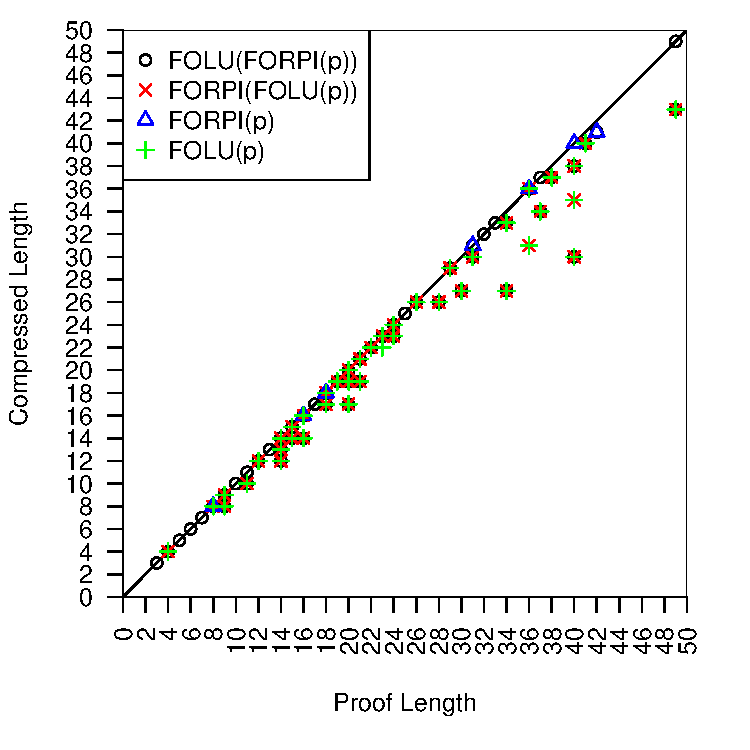
\includegraphics[scale=0.5]{images/everything-forpi-folu-length_vs_compress_length_all_proofs.pdf}}}
%    \subfloat[Compressed length against input length (resolutions)]{{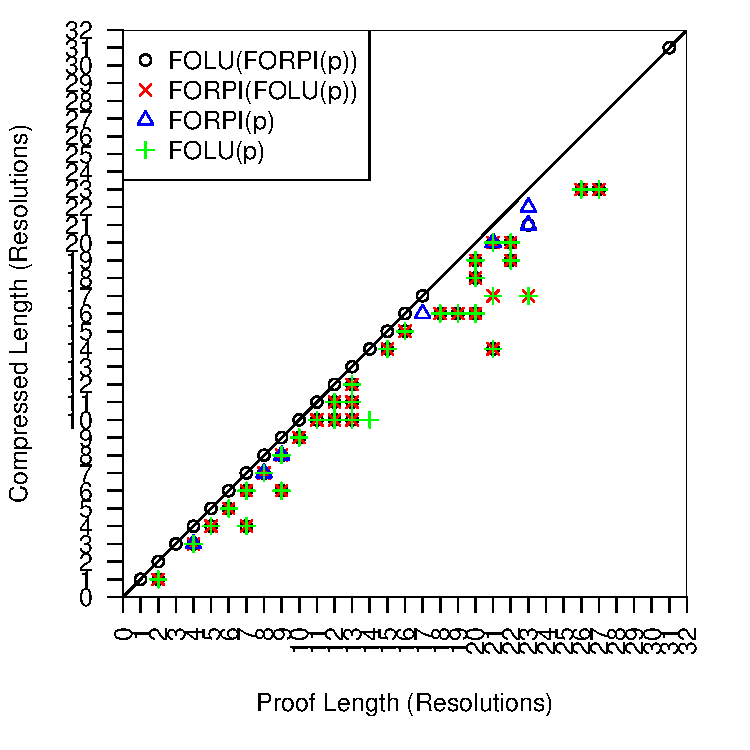
\includegraphics[scale=0.5]{images/everything-forpi-folu-res_length_vs_compress_res_length_all_proofs.pdf} }}
\subfloat[\FORPI(\GFOLU(p)) vs. \GFOLU(\FORPI(p))]{{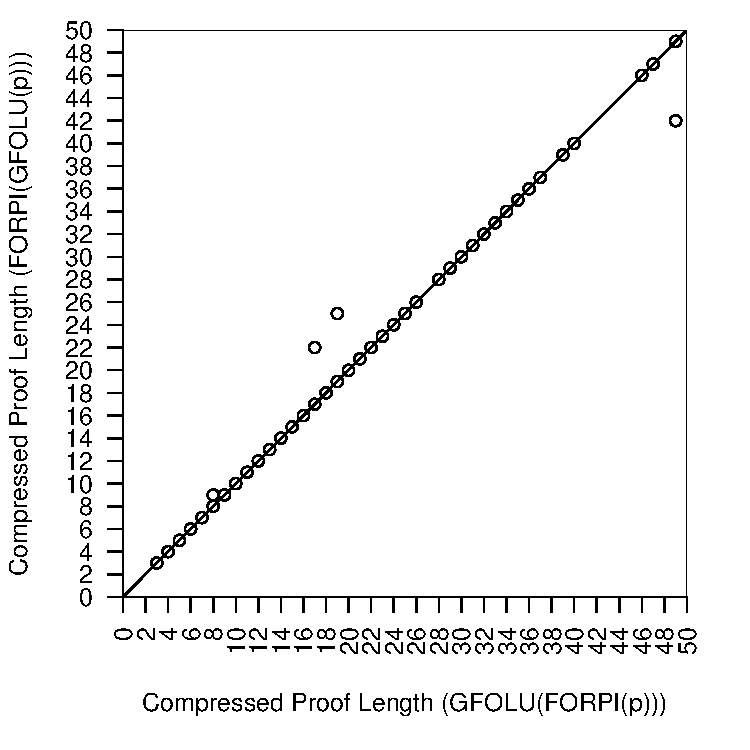
\includegraphics[scale=0.5]{images/forpi-folu-vs-folu-forpi-length_vs_compress_length_all_proofs.pdf} }}
\caption{Experimental results}
\label{fig:ex}
\end{figure}





\section{Conclusions and Future Work}\label{sec:conclusion}

The main contribution of this paper is the generalization of the propositional proof compression algorithm {\RPI} to the first-order case. As indicated in Section \ref{sec:Challenges}, the generalization is challenging, because unification changes the pivots and, consequently, must be taken into account when collecting safe literals and marking nodes for deletion.

Every computational experiment evaluates not only the algorithm but also the data on which it is executed. Although the experimental results are not as promissing as expected, this is due to the fact that the 308 proofs currently available are too short to contain a significant amount of irregularities. This is a valuable piece of information, allowing us to conclude that it is not worth applying {\FORPI} to pure resolution proofs which current state-of-the-art first-order theorem provers seem capable of producing. Nevertheless, based on our positive results for {\RPI} on much longer proofs generated by SAT and SMT solvers \cite{LURPI}, {\FORPI} remains a promising option to be revisited in the future, when the performance of first-order theorem provers catch up with advances in SAT and SMT and taller first-order benchmark proofs become available.

% These algorithms are very fast, and together they may simplify the proof considerably for a relatively quick time cost.

% {\RPI} performs best when the proofs are tall; {\FORPI} will likely perform similarly. However, the proofs in this data set are relatively short, and those compressed by {\GFOLU} first are even shorter. Thus, the performance of {\FORPI} is not surprising.

%{\FORPI} continues to support the idea of listing propositional proof compression algorithms to the first-order case. The experimental results discussed in the previous continue to be encouraging, and are consistent with trends observed in the propositional case. 

%\paragraph{Acknowledgments:}


\begin{footnotesize}
%\bibliographystyle{splncs}
\bibliographystyle{plain}
\bibliography{biblio}
\end{footnotesize}
\appendix
\section{Algorithm \texttt{RecyclePivotsWithIntersection}}
\label{Section:RPI}

\newcommand{\tRes}{\odot}
\newcommand{\tResFact}{\otimes}
\newcommand{\tResChain}{\ominus}
\newcommand{\AXC}{\AxiomC}
\newcommand{\BIC}{\BinaryInfC}
\newcommand{\RName}[1]{\RightLabel{#1}}
\newcommand{\p}[1]{\hat{#1}}
\newcommand{\ub}[2]{\underbrace{#1}_{#2}}
\newcommand{\tResStar}{\circledast}

\texttt{RecyclePivotsWithIntersection} ({\RPI}) \cite{LURPI} aims at compressing irregular proofs. It can be seen as a simple 
but significant modification of the {\RP} algorithm described in 
\cite{RP08}, 
from which it derives its name. 
Although in the worst case full regularization can increase the proof length exponentially 
\cite{Tseitin}, these algorithms show that 
many irregular proofs can have their length decreased if a careful partial regularization is performed. 

Consider an irregular proof of the form $\psi[ \eta \tRes_p \psi'[\eta' \tRes_p \eta''] ]$ and assume, without loss of generality, that $p \in \eta$ and $p \in \eta'$. Then, if $\eta' \tRes_p \eta''$ is replaced by $\eta''$ within the proof-context $\psi'[\ ]$, the clause $\eta \tRes_p \psi'[\eta'']$ subsumes the clause $\eta \tRes_p \psi'[\eta' \tRes_p \eta'']$, because even though the literal $\neg p$ of $\eta''$ is
propagated down, it gets resolved against the literal $p$ of $\eta$ later on below in the proof. More precisely, even though it might be the case that $\neg p \in \psi'[\eta'']$ while $\neg p \notin \psi'[\eta' \tRes_p \eta'']$, it is necessarily the case that $\neg p \notin \eta \tRes_p \psi'[\eta' \tRes_p \eta'']$ and $\neg p \notin \eta \tRes_p \psi'[\eta'']$.

Although the remarks above suggest that it is safe to replace $\eta' \tRes_p
\eta''$ by $\eta''$ within the proof-context $\psi'[\ ]$, this is not always the
case. If a node in $\psi'[\ ]$ has a child in $\psi[\ ]$, then the literal $\neg
p$ might be propagated down to the root of the proof, and hence, the clause
$\psi[ \eta \tRes_p \psi'[ \eta''] ]$ might not subsume the clause $\psi[ \eta
\tRes_p \psi'[\eta' \tRes_p \eta''] ]$. Therefore, it is only safe to do the
replacement if the literal $\neg p$ gets resolved in all paths from $\eta''$ to the root or if it already occurs in the root clause of the original proof $\psi[ \eta \tRes_p \psi'[\eta' \tRes_p \eta''] ]$.


\begin{algorithm}[bt]
\begin{footnotesize}
\SetKwInOut{Input}{input}\SetKwInOut{Output}{output}
\SetKwData{units}{unitsQueue}
\SetKwData{fixedUnits}{fixedUnitsQueue}

\Input{A proof $\psi$}
\Output{A possibly less-irregular proof $\psi'$}

\BlankLine

$\psi'$ $\la$ $\psi$\;
traverse $\psi'$ bottom-up and \ForEach{node $\eta$ in $\psi'$}{
   % \uIf{$\eta$ is an input node}{ 
   % 		do nothing \;
   %  }
   %  \ElseIf{$\eta$ is a resolvent node}{
   %   setSafeLiterals($\eta$) \;
   %   regularizeIfPossible($\eta$)
   % }
%% SM: original version: do we really need the "do nothing" branch?
   \If{$\eta$ is a resolvent node}{
     setSafeLiterals($\eta$) \;
     regularizeIfPossible($\eta$)
   }
  }
$\psi'$ $\la$ fix($\psi'$) \;
\Return {$\psi'$}\;
\caption{\label{algo:RPI} \texttt{\RPI}}
\end{footnotesize}
\end{algorithm}

%\begin{code}
%  function recyclePivotsWithIntersection(p: Proof): Proof = {
%    traverseBottomUp(p)(
%      n => {
%        if (n is Input) doNothing
%        else if (n is Resolvent) {
%          setSafeLiterals(n)
%          regularizeIfPossible(n)
%          for (c in n.children) c.freeMemory
%        } 
%      }
%    )
%    fix(p)  
%  }
%\end{code}

These observations lead to the idea of traversing the proof in a bottom-up
manner, storing for every node a set of \emph{safe literals} that get resolved
in all paths below it in the proof (or that already occurred in the root clause
of the original proof). Moreover, if one of the node's resolved literals belongs
to the set of safe literals, then it is possible to regularize the node by
replacing it by one of its parents (cf.\ Algorithm~\ref{algo:RPI}). 

The regularization of a node should replace a node by one of its parents, and more precisely by the parent whose clause contains the resolved literal that is safe. After regularization, all nodes below the regularized node may have to be fixed. However, since the regularization is done with a bottom-up traversal, and only nodes below the regularized node need to be fixed, it is again possible to postpone fixing and do it with only a single traversal afterwards. 
Therefore, instead of replacing the irregular node by one of its parents immediately, 
its other parent is replaced by \texttt{deletedNodeMarker}, as shown in Algorithm~\ref{algo:Regularize}. Only later during fixing, 
the irregular node is actually replaced by its surviving parent (i.e. the parent that is not \texttt{deletedNodeMarker}).



\begin{algorithm}[p]
\begin{footnotesize}
\SetKwInOut{Input}{input}\SetKwInOut{Output}{output}
\SetKwData{units}{unitsQueue}
\SetKwData{fixedUnits}{fixedUnitsQueue}

\Input{A node $\eta$}
\Output{nothing (but the proof containing $\eta$ may be changed)}

\BlankLine
    \uIf{$\eta${\upshape.rightResolvedLiteral} $\in$ $\eta${\upshape.safeLiterals}}{
      replace left parent of $\eta$ by \texttt{deletedNodeMarker} \;
      mark $\eta$ as regularized
    }
    \ElseIf{\textrm{$\eta${\upshape.leftResolvedLiteral} $\in$ $\eta${\upshape.safeLiterals}}}{
      replace right parent of $\eta$ by \texttt{deletedNodeMarker} \;
      mark $\eta$ as regularized
    }
\caption{\label{algo:Regularize} \texttt{regularizeIfPossible}}
\end{footnotesize}
\end{algorithm}



\begin{algorithm}[p]
\begin{footnotesize}
\SetKwInOut{Input}{input}\SetKwInOut{Output}{output}
\SetKwData{units}{unitsQueue}
\SetKwData{fixedUnits}{fixedUnitsQueue}

\Input{A node $\eta$}
\Output{nothing (but the node $\eta$ gets a set of safe literals)}

\BlankLine

    \uIf{$\eta$ is a root node with no children}{
      $\eta$.safeLiterals $\la$ $\eta$.clause  
    }
    \Else{
      \ForEach{$\eta'$ $\in$ $\eta${\upshape.children}}{
        \uIf{$\eta'$ is marked as regularized}{ 
          safeLiteralsFrom($\eta'$) $\la$ $\eta'$.safeLiterals \;}
        \uElseIf{$\eta$ is left parent of $\eta'$}{ 
        	safeLiteralsFrom($\eta'$) $\la$ $\eta'$.safeLiterals $\cup$ \{ $\eta'$.rightResolvedLiteral \} \;
        }
        \ElseIf{$\eta$ is right parent of $\eta'$}{ 
			safeLiteralsFrom($\eta'$) $\la$ $\eta'$.safeLiterals $\cup$ \{ $\eta'$.leftResolvedLiteral \} \;
        }
      }
      $\eta$.safeLiterals $\la$ $\bigcap_{\eta' \in \eta\textrm{.children}}$ safeLiteralsFrom($\eta'$)
    }
\caption{\label{algo:SetSafeLiterals} \texttt{setSafeLiterals}}
\end{footnotesize}
\end{algorithm}

%\begin{code}
%  function setSafeLiterals(n: Resolvent) = {
%    if (n is a root node with no children) {
%      n.safeLiterals = n.clause  
%    }
%    else {
%      val safeLiteralsPerChild = for (c in n.children) yield {
%        if (c is marked as regularized) c.safeLiterals 
%        else if (c.left == n) c.safeLiterals $+cup$ {c.resolvedLiterals.right}
%        else if (c.right == n) c.safeLiterals $+cup$ {c.resolvedLiterals.left}
%      }
%      n.safeLiterals = intersection(safeLiteralsPerChild)
%    }
%  }
%\end{code}

The set of safe literals of a node $\eta$ can be computed from the set of safe
literals of its children (cf.\ Algorithm~\ref{algo:SetSafeLiterals}). In the case when $\eta$ has a single child $\varsigma$, the safe literals of $\eta$ are simply the safe literals of $\varsigma$ together with the resolved literal $p$ of $\varsigma$ belonging to $\eta$ ($p$ is safe for $\eta$, because whenever $p$ is propagated down the proof through $\eta$, $p$ gets resolved in $\varsigma$). It is important to note, however, that if $\varsigma$ has been marked as regularized, it will eventually be replaced by $\eta$, and hence $p$ should not be added to the safe literals of $\eta$. In this case, the safe literals of $\eta$ should be exactly the same as the safe literals of $\varsigma$. When $\eta$ has several children, the safe literals of $\eta$ w.r.t. a child $\varsigma_i$ contain literals that are safe on all paths that go from $\eta$ through $\varsigma_i$ to the root. For a literal to be safe for all paths from $\eta$ to the root, it should therefore be in the intersection of the sets of safe literals w.r.t. each child.


The {\RP} and the {\RPI} algorithms differ from each other mainly in the
computation of the safe literals of a node that has many children. While {\RPI}
returns the intersection as shown in Algorithm~\ref{algo:SetSafeLiterals}, {\RP}
returns the empty set (cf.\ Algorithm~\ref{algo:SetSafeLiteralsRP}). Additionally, while in {\RPI} the safe literals of the root node contain all the literals of the root clause, in {\RP} the root node is always assigned an empty set of literals. 
(Of course, this makes a difference only when the proof is not a refutation.)
Note that during a traversal of the proof, 
the lines from 5 to 10 in Algorithm~\ref{algo:SetSafeLiterals} are executed as many times as the number of edges in the proof. 
Since every node has at most two parents, the number of edges is at most twice the number of nodes. 
Therefore, during a traversal of a proof with $n$ nodes, lines from 5 to 10 are
executed at most $2n$ times, and the algorithm remains linear.
In our prototype implementation, the sets of safe literals are instances of Scala's 
\texttt{mutable.HashSet} class. Being mutable, new elements can be added efficiently.
And being HashSets, membership checking is done in constant time in the average case, 
and set intersection (line 12) can be done in $O(k.s)$, where $k$ is the number of sets and $s$ is the size of the smallest set.



\begin{algorithm}[p]
\begin{footnotesize}
\SetKwInOut{Input}{input}\SetKwInOut{Output}{output}
\SetKwData{units}{unitsQueue}
\SetKwData{fixedUnits}{fixedUnitsQueue}

\Input{A node $\eta$}
\Output{nothing (but the node $\eta$ gets a set of safe literals)}

\BlankLine

    \uIf{$\eta$ is a root node with no children}{
      $\eta$.safeLiterals $\la$ $\emptyset$ 
    }
    \Else{
      \uIf{$\eta$ has only one child $\eta'$}{
        \uIf{$\eta'$ is marked as regularized}{ 
          $\eta$.safeLiterals $\la$ $\eta'$.safeLiterals \;}
        \uElseIf{$\eta$ is left parent of $\eta'$}{ 
        	$\eta$.safeLiterals $\la$ $\eta'$.safeLiterals $\cup$ \{ $\eta'$.rightResolvedLiteral \} \;
        }
        \ElseIf{$\eta$ is right parent of $\eta'$}{ 
			$\eta$.safeLiterals $\la$ $\eta'$.safeLiterals $\cup$ \{ $\eta'$.leftResolvedLiteral \} \;
        }
      }
      \Else{
      	$\eta$.safeLiterals $\la$ $\emptyset$
      }
    }
\caption{\label{algo:SetSafeLiteralsRP} \texttt{setSafeLiterals} for \RP}
\end{footnotesize}
\end{algorithm}

%
%\begin{code}
%  function setSafeLiterals(n: Resolvent) = {
%     n.safeLiterals = 
%       if (n has only one child c) {
%         if (c is marked as regularized) c.safeLiterals 
%         else if (c.left == n) c.safeLiterals $+cup$ {c.resolvedLiterals.left}
%         else if (c.right == n) c.safeLiterals $+cup$ {c.resolvedLiterals.right}
%       }
%       else $+emptyset$
%  }
%\end{code}



%\begin{example}
When applied to the proof $\psi$ shown in Example \ref{Example:Proof}, the algorithm {\RPI} assigns $\{a,c\}$ and $\{a, \neg c\}$ as the safe literals of, respectively, $\eta_5$ and $\eta_8$. The safe literals of $\eta_4$ w.r.t. its children $\eta_5$ and $\eta_8$ are respectively $\{a,c,b\}$ and $\{a, \neg c, b\}$, and hence the safe literals of $\eta_4$ are $\{a,b\}$ (the intersection of $\{a,c,b\}$ and $\{a, \neg c, b\}$). Since the right resolved literal of $\eta_4$ ($a$) belongs to $\eta_4$'s safe literals, $\eta_4$ is correctly detected as a redundant node and hence regularized: $\eta_4$ is replaced by its right parent $\eta_3$. The resulting proof is shown below:

\begin{small}
\begin{prooftree}
\AXC{$ \eta_1: \neg a $}
		\AXC{$ \eta_2: a, c, \neg b $}
						\AXC{$ \eta_3:  a, b $}\RName{$ $}
			\BIC{$ \eta_5: a, c$}	\RName{$ $}
	\BIC{$\eta_6: c$}
		\AXC{$ \eta_3 $}
				\AXC{$ \eta_7: a, \neg c, \neg b $} \RName{$ $}
			\BIC{$ \eta_8: a, \neg c$}	\RName{$ $}
					\AXC{$ \eta_1 $}  \RName{$ $}
				\BIC{$ \eta_9: \neg c$}	\RName{$ $}
		\BIC{$\psi: \bot$}	
\end{prooftree}
\end{small}

%This proof corresponds to the proof term
$$
(\ub{\{\neg a\}}{\eta_1} \tRes (\{a, c, \neg b\} \tRes \ub{\{a, b\}}{\eta_3})) \tRes ((\eta_3 \tRes \{\neg b, \neg c, a\}) \tRes \eta_1)
$$
%
\noindent%
{\RP}, on the other hand, assigns $\emptyset$ as the set of safe literals for $\eta_4$. Therefore, it does not detect that $\eta_4$ is a redundant irregular node, and then $\RP(\varphi) = \varphi$. 
 %
\hfill\QED
\end{example}

\begin{theorem}
\label{Theorem:RPIBetterThanRP}
For any proof $\varphi$, $|\RPI(\varphi)| \leq |\RP(\varphi)|$.
\end{theorem}
\begin{proof}
  For every node $\eta$ in $\varphi$, let $S^{\eta}_{\RPI}$ (resp.,
  $S^{\eta}_{\RP}$) be the set of safe literals for $\eta$ computed by {\RPI} and
  {\RP}. It is easy to see that $S^{\eta}_{\RPI} \supseteq S^{\eta}_{\RP}$ for all
  $\eta$. Therefore, {\RPI} detects and eliminates more redundancies than {\RP}.
%
\hfill\QED
\end{proof}

The better compression of {\RPI} does not come for free, 
as computing an intersection of sets is more costly than assigning the empty set. 
For a node $\eta$ with $k$ children, $k$ sets must be intersected and the size of each set is 
in the worst case in $O(h)$, where $h$ is the length of the shortest path from $\eta$ to a root.






\end{document}

% vim: tw=100
